\chapter{Testing}

Il software \`{e} stato testato con successo sui sistemi operativi \textit{Windows 10}, \textit{Ubuntu 16.04} e \textit{Mac OSx El Capitan}.  

\vspace*{0.5cm}
Sono di seguito presentati esempi del file di configurazione (\textbf{Figura \ref{fig:conf}}), del file contenente le informazioni di sistema (\textbf{Figura \ref{fig:sys_info}}) e del file di log (\textbf{Figura \ref{fig:log}}).

\vspace*{0.5cm}
\begin{figure}[htp]
\centering
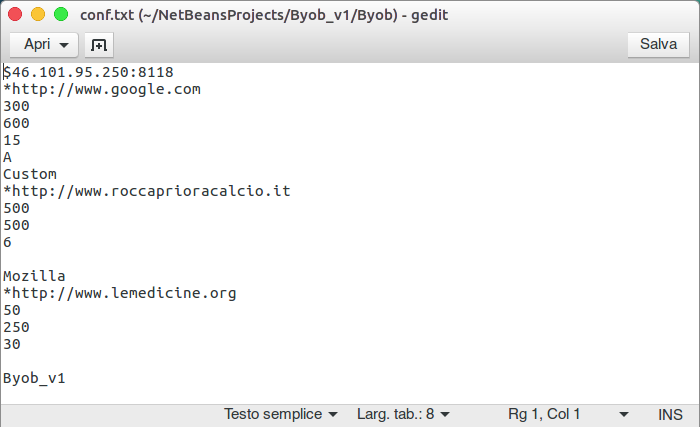
\includegraphics[width=0.7\linewidth]{imgs/conf}
\caption{File di configurazione}
\label{fig:conf}
\end{figure}

\begin{figure}[htp]
\centering
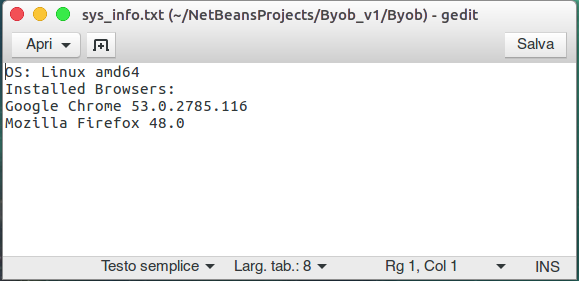
\includegraphics[width=0.7\linewidth]{imgs/sys_info}
\caption{Informazioni del Sistema}
\label{fig:sys_info}
\end{figure}

\begin{figure}[htp]
\centering
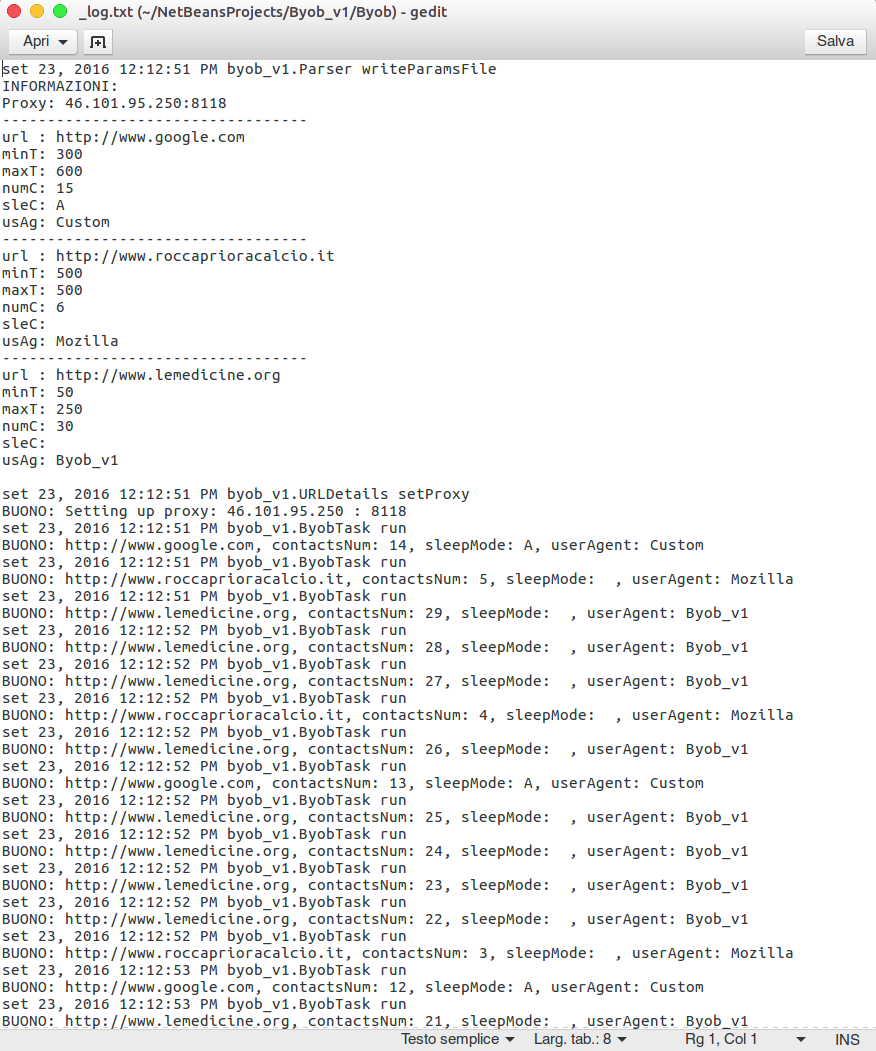
\includegraphics[width=0.7\linewidth]{imgs/log}
\caption{File di log}
\label{fig:log}
\end{figure}

\newpage
La verifica dei contatti avvenuti con le \textit{URL} specificate \`{e} stato facilitato dall'utilizzo di un software di monitoraggio grafico della rete chiamato \textit{EtherApe}\footnote{http://etherape.sourceforge.net/}

\vspace{0.5cm}
\begin{figure}[htp]
\centering
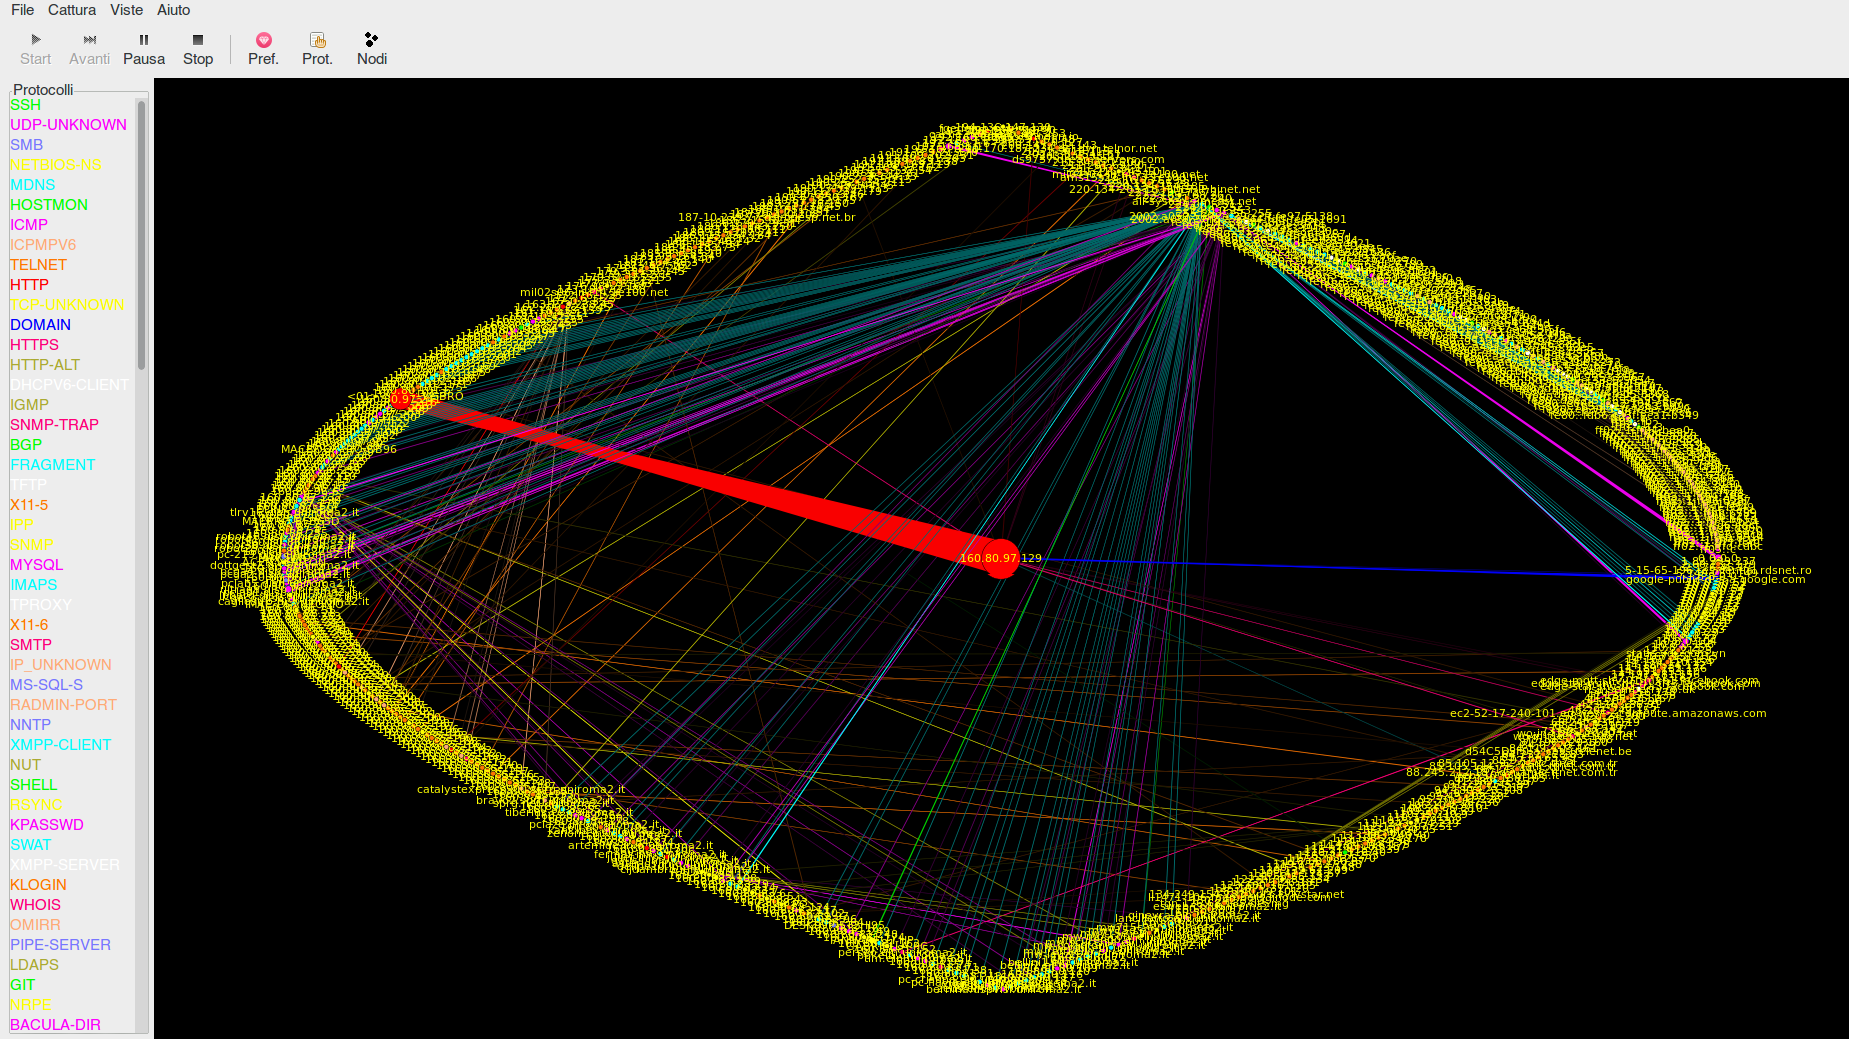
\includegraphics[width=1\linewidth]{imgs/etherape}
\caption{Graphical network monitor: etherApe}
\label{fig:etherape}
\end{figure}

